\documentclass{article}\usepackage{graphicx, color}
%% maxwidth is the original width if it is less than linewidth
%% otherwise use linewidth (to make sure the graphics do not exceed the margin)
\makeatletter
\def\maxwidth{ %
  \ifdim\Gin@nat@width>\linewidth
    \linewidth
  \else
    \Gin@nat@width
  \fi
}
\makeatother

\definecolor{fgcolor}{rgb}{0.2, 0.2, 0.2}
\newcommand{\hlnumber}[1]{\textcolor[rgb]{0,0,0}{#1}}%
\newcommand{\hlfunctioncall}[1]{\textcolor[rgb]{0.501960784313725,0,0.329411764705882}{\textbf{#1}}}%
\newcommand{\hlstring}[1]{\textcolor[rgb]{0.6,0.6,1}{#1}}%
\newcommand{\hlkeyword}[1]{\textcolor[rgb]{0,0,0}{\textbf{#1}}}%
\newcommand{\hlargument}[1]{\textcolor[rgb]{0.690196078431373,0.250980392156863,0.0196078431372549}{#1}}%
\newcommand{\hlcomment}[1]{\textcolor[rgb]{0.180392156862745,0.6,0.341176470588235}{#1}}%
\newcommand{\hlroxygencomment}[1]{\textcolor[rgb]{0.43921568627451,0.47843137254902,0.701960784313725}{#1}}%
\newcommand{\hlformalargs}[1]{\textcolor[rgb]{0.690196078431373,0.250980392156863,0.0196078431372549}{#1}}%
\newcommand{\hleqformalargs}[1]{\textcolor[rgb]{0.690196078431373,0.250980392156863,0.0196078431372549}{#1}}%
\newcommand{\hlassignement}[1]{\textcolor[rgb]{0,0,0}{\textbf{#1}}}%
\newcommand{\hlpackage}[1]{\textcolor[rgb]{0.588235294117647,0.709803921568627,0.145098039215686}{#1}}%
\newcommand{\hlslot}[1]{\textit{#1}}%
\newcommand{\hlsymbol}[1]{\textcolor[rgb]{0,0,0}{#1}}%
\newcommand{\hlprompt}[1]{\textcolor[rgb]{0.2,0.2,0.2}{#1}}%

\usepackage{framed}
\makeatletter
\newenvironment{kframe}{%
 \def\at@end@of@kframe{}%
 \ifinner\ifhmode%
  \def\at@end@of@kframe{\end{minipage}}%
  \begin{minipage}{\columnwidth}%
 \fi\fi%
 \def\FrameCommand##1{\hskip\@totalleftmargin \hskip-\fboxsep
 \colorbox{shadecolor}{##1}\hskip-\fboxsep
     % There is no \\@totalrightmargin, so:
     \hskip-\linewidth \hskip-\@totalleftmargin \hskip\columnwidth}%
 \MakeFramed {\advance\hsize-\width
   \@totalleftmargin\z@ \linewidth\hsize
   \@setminipage}}%
 {\par\unskip\endMakeFramed%
 \at@end@of@kframe}
\makeatother

\definecolor{shadecolor}{rgb}{.97, .97, .97}
\definecolor{messagecolor}{rgb}{0, 0, 0}
\definecolor{warningcolor}{rgb}{1, 0, 1}
\definecolor{errorcolor}{rgb}{1, 0, 0}
\newenvironment{knitrout}{}{} % an empty environment to be redefined in TeX

\usepackage{alltt}
\usepackage[utf8]{inputenc}
\usepackage{graphicx}
\usepackage[colorlinks=true,urlcolor=blue]{hyperref}
\usepackage{array}
\usepackage{color}
\usepackage[english]{babel}
\usepackage{amsfonts}
\usepackage{url}
\usepackage{bm}
\usepackage[margin=2.5cm]{geometry}

\newcommand{\R}{\mathbb{R}}
\newcommand{\beq}{\begin{equation}}
\newcommand{\eeq}{\end{equation}}
\newcommand{\m}[1]{\mathbf{#1}}

\title{Test of id\_spatial\_sim}
\author{Steven Riley}
\date{\today}

\sloppy
\hyphenpenalty 10000

%%%%%%%%%%%%%%%%%%%%%%%%%%%%%%%%%%%%%%%%%%%%%%%%%%
%%%%%%%%%%%%%%%%%%%%%%%%%%%%%%%%%%%%%%%%%%%%%%%%%%
%%%%%%%%%%%%%%%%%%%%%%%%%%%%%%%%%%%%%%%%%%%%%%%%%%
\IfFileExists{upquote.sty}{\usepackage{upquote}}{}
\begin{document}
\selectlanguage{english}

%% some knitr options



\maketitle




\newpage
%%%%%%%%%%%%%%%%%%%%%%%%%%%%%%%%%%%%%%%%%%%%%%%%%%
%%%%%%%%%%%%%%%%%%%%%%%%%%%%%%%%%%%%%%%%%%%%%%%%%%
%%%%%%%%%%%%%%%%%%%%%%%%%%%%%%%%%%%%%%%%%%%%%%%%%%

%%%%%%%%%%%%%%%%%%%%%%%%%%
%%%%%%%%%%%%%%%%%%%%%%%%%%
\section{Playing around with the ebola library}
%%%%%%%%%%%%%%%%%%%%%%%%%%
%%%%%%%%%%%%%%%%%%%%%%%%%%

When this is not being run in bacth mode, we need to set the working directoy.
This appears here as a comment, so it is not run when in batch mode.

\begin{knitrout}
\definecolor{shadecolor}{rgb}{0.969, 0.969, 0.969}\color{fgcolor}\begin{kframe}
\begin{alltt}
\hlcomment{# setwd("~/Dropbox/git/id_spatial_sim/testsuite")}
\end{alltt}
\end{kframe}
\end{knitrout}


First we declare some packages that we will use below.

\begin{knitrout}
\definecolor{shadecolor}{rgb}{0.969, 0.969, 0.969}\color{fgcolor}\begin{kframe}
\begin{alltt}
\hlfunctioncall{require}(\hlstring{"raster"})
\end{alltt}


{\ttfamily\noindent\itshape\color{messagecolor}{\#\# Loading required package: raster}}

{\ttfamily\noindent\itshape\color{messagecolor}{\#\# Loading required package: methods}}

{\ttfamily\noindent\itshape\color{messagecolor}{\#\# Loading required package: sp}}\end{kframe}
\end{knitrout}


The first line of the batch file builds a synthetic population with density
proportional the ebola affected region in west Africa, but much smaller. With a total population of only
100,000. Each person has, one average, 10 network links but these links are
distributed entirely randomly in space. This takes a while because the
average population is very low and there is high variability. Hence the
accept-reject method for assinging nodes has many rejection steps. We assume
that only one individual lives in a household for this population. 

%% <<>>=
%% # system("../g++/ebola_build.exe ./params/fast_test_build_params.in ./output/small_pop1")  
%% @

The second line of the batch file runs an outbreak of only two generations 20
times. The outbreak is seeded in the same area as the reported patient zero for
the 2014 Ebola outbreak. There are 4 iniitally infectious individuals at time
$t=0$. Transmission is only via the spatial kernel and thus allows us to test
that the basic reproductive number is parameterized correctly. We can also
report the serial interval.

We first load the linelist of events from all the realizations. And check the
dimensions of the output. The output was designed before csvs became so
dominant!

\begin{knitrout}
\definecolor{shadecolor}{rgb}{0.969, 0.969, 0.969}\color{fgcolor}\begin{kframe}
\begin{alltt}
dat0 <- \hlfunctioncall{read.table}(file=\hlstring{"./output/ft_sp_pset_0_Events.out"},header=TRUE)
dimDat0 <- \hlfunctioncall{dim}(dat0)
noevents <- dimDat0[1]
nocols <- dimDat0[2]
\end{alltt}
\end{kframe}
\end{knitrout}


The column headings describe the information captured in the event file
\begin{knitrout}
\definecolor{shadecolor}{rgb}{0.969, 0.969, 0.969}\color{fgcolor}\begin{kframe}
\begin{alltt}
\hlfunctioncall{names}(dat0)
\end{alltt}
\begin{verbatim}
##  [1] "Run"        "Day"        "Event"      "Index"      "X"         
##  [6] "Y"          "Generation" "infector"   "infect_x"   "infect_y"
\end{verbatim}
\end{kframe}
\end{knitrout}


We can subset these 'data' to look at only infection. Then examine the number of
infections by generation for each realization.

\begin{knitrout}
\definecolor{shadecolor}{rgb}{0.969, 0.969, 0.969}\color{fgcolor}\begin{kframe}
\begin{alltt}
tabInfs0 <- dat0[dat0$Event==0,]
\hlfunctioncall{table}(tabInfs0$Run,tabInfs0$Generation)
\end{alltt}
\begin{verbatim}
##    
##      1  2
##   0  4  5
##   1  4  0
##   2  4  5
##   3  4 12
##   4  4  8
##   5  4  8
##   6  4 11
##   7  4 14
##   8  4 11
##   9  4  2
\end{verbatim}
\end{kframe}
\end{knitrout}


And look at the average number in the second generation divided by the number of
seeds as a test of the $R_0$ parameterization. 

\begin{knitrout}
\definecolor{shadecolor}{rgb}{0.969, 0.969, 0.969}\color{fgcolor}\begin{kframe}
\begin{alltt}
\hlfunctioncall{table}(tabInfs0$Generation)[2]/\hlfunctioncall{table}(tabInfs0$Generation)[1]
\end{alltt}
\begin{verbatim}
##   2 
## 1.9
\end{verbatim}
\end{kframe}
\end{knitrout}


Its difficult to tell if this is accurate with such small numbers, so we can
load up the similar run with 100 realisations.

\begin{knitrout}
\definecolor{shadecolor}{rgb}{0.969, 0.969, 0.969}\color{fgcolor}\begin{kframe}
\begin{alltt}
dat1 <- \hlfunctioncall{read.table}(file=\hlstring{"./output/ft_sp_pset_1_Events.out"},header=TRUE)
\hlfunctioncall{dim}(dat1)
\end{alltt}
\begin{verbatim}
## [1] 4264   10
\end{verbatim}
\begin{alltt}
tabInfs1 <- dat1[dat1$Event==0,]
estR0 <- \hlfunctioncall{table}(tabInfs1$Generation)[2] / \hlfunctioncall{table}(tabInfs1$Generation)[1]
estR0
\end{alltt}
\begin{verbatim}
##     2 
## 1.665
\end{verbatim}
\end{kframe}
\end{knitrout}


Might also be worth looking at the distribution of the ratio of secondary cases
for each realization. So we make a table of generations by run and plot a
histogram of the ratios for each realization. You can see quite a bit of
variance in the size of the second generation of this model. Note that the
offspring distribution will be even more highly over-dispersed because these
results are based on a seed of 4.

\begin{knitrout}
\definecolor{shadecolor}{rgb}{0.969, 0.969, 0.969}\color{fgcolor}\begin{kframe}
\begin{alltt}
tabRunGen1 <- \hlfunctioncall{table}(tabInfs1$Run,tabInfs1$Generation)
\hlfunctioncall{hist}( tabRunGen1[,2]/tabRunGen1[,1],breaks=\hlfunctioncall{seq}(0,7,0.25),
      xlab=\hlstring{"Ratio first to second gens"},main=\hlstring{""})
\hlfunctioncall{abline}(v=estR0,lwd=2,col=\hlstring{"red"})	
\end{alltt}
\end{kframe}

{\centering 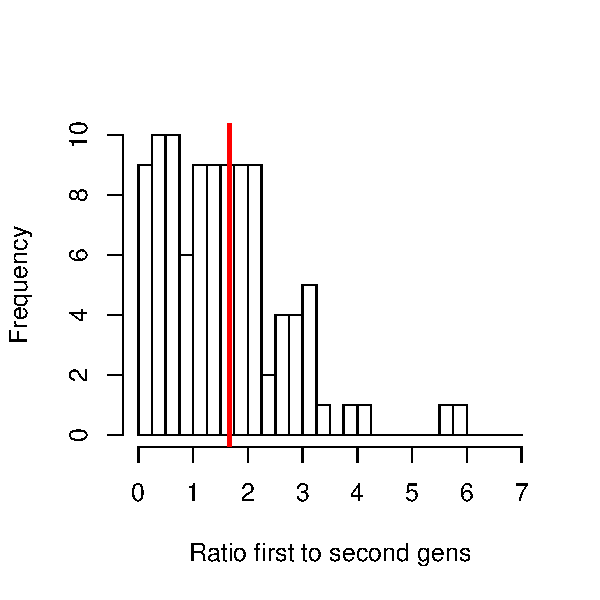
\includegraphics[width=\textwidth]{figs/unnamed-chunk-10} 

}



\end{knitrout}


It is also straightforward to look at the distributions of different waiting
times in the model because we 'observe' them directly in this idealized
linelist. So the average serial interval is equal to the average time of the
infection event in the second generation.

\begin{knitrout}
\definecolor{shadecolor}{rgb}{0.969, 0.969, 0.969}\color{fgcolor}\begin{kframe}
\begin{alltt}
vecTimesG1 <- tabInfs1[tabInfs1$Generation==2,\hlstring{"Day"}] 
\hlfunctioncall{mean}(vecTimesG1)
\end{alltt}
\begin{verbatim}
## [1] 16.51
\end{verbatim}
\begin{alltt}
\hlfunctioncall{hist}(vecTimesG1,breaks=\hlfunctioncall{seq}(0,50,2),main=\hlstring{""},
    xlab=\hlstring{"Time from exposure to \hlfunctioncall{infection} (2 day bins)"})
\end{alltt}
\end{kframe}

{\centering 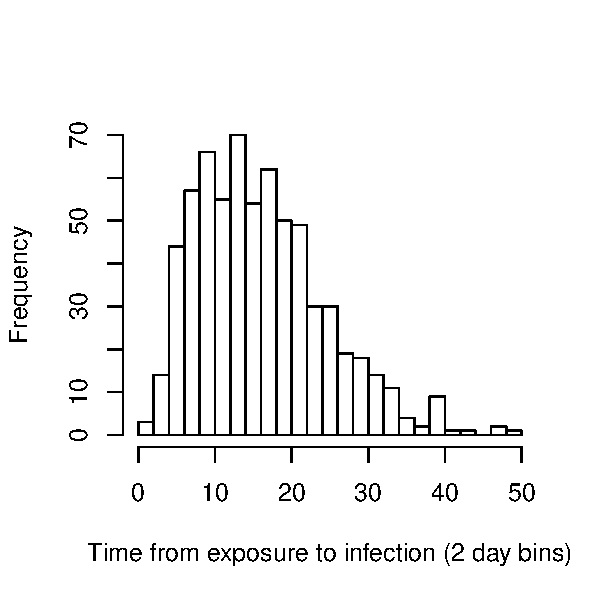
\includegraphics[width=\textwidth]{figs/unnamed-chunk-11} 

}



\end{knitrout}


Its a highly over-dospersed distribution, suggesting that events such as the
long time from exposure to infection for the non-African infection event
in Spain are not entirely inconsistent with the NEJM estimated parameters.

\subsection{Spatial analysis}

Next we load up the population desity on which the model was based and look at
the spatial distribution of these initial infections.

\end{document}

